% schéma de comparaison des formats QHD et TVSD

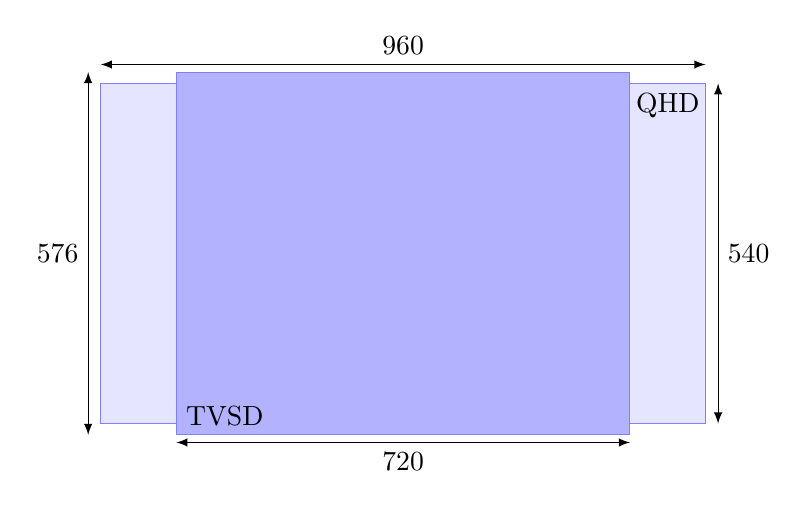
\begin{tikzpicture}[scale=.8]
\filldraw[draw=blue!50,fill=blue!10] (-4.8,-2.7) rectangle (4.8,2.7);
\filldraw[draw=blue!50,fill=blue!30] (-3.6,-2.88) rectangle (3.6,2.88);
% \draw[draw=blue!50] (-4.8,-2.7) rectangle (4.8,2.7);
\draw	(-3.6,-2.88) node[anchor=south west] {TVSD}
			(4.2,2.7) node[anchor=north] {QHD};

% QHD
\draw [<->,latex-latex] (5,-2.7) -- node[anchor=west] {540} (5,2.7);
\draw [<->,latex-latex] (-4.8,3) -- node[anchor=south] {960} (4.8,3);

% TVSD
\draw [<->,latex-latex] (-5,-2.88) -- node[anchor=east] {576} (-5,2.88);
\draw [<->,latex-latex] (-3.6,-3) -- node[anchor=north] {720} (3.6,-3);

\end{tikzpicture}